%================================================
% CHAPTER 2: STATE OF THE ART AND REQUIREMENTS SPECIFICATION
% ATB BI PROJECT — English version aligned with NotMychapter2 structure
%================================================
\chapter{State of the Art and Requirements Specification}

\section{Introduction}

This chapter establishes the theoretical and functional foundations of the ATB Business
Intelligence and Machine Learning project. It is structured around three objectives:
(1) to position the project within the existing scientific literature on Business Intelligence,
machine learning, data warehousing, and MLOps; (2) to justify every architectural and
algorithmic choice through a systematic review of the relevant technical domains; and
(3) to provide the operational conceptual framework used to design the ATB BI platform,
from raw CSV ingestion to supervised risk classification and interactive dashboarding.

The approach follows the structure recommended by our academic supervisor: general concepts
and state of the art are presented first, followed by their specific application to the
banking sector and to this project, ensuring that the chapter is understandable to a reader
unfamiliar with the field.


%================================================
\section{State of the Art: Fundamentals}
%================================================

%----------------------------------------------
\subsection{Business Intelligence: Definitions and Domains}
%----------------------------------------------

Business Intelligence (BI) refers to the set of methodologies, architectures, tools, and
processes used to transform raw operational data into reliable, structured information
supporting managerial decision-making \cite{chaudhuri2011}. According to Chaudhuri et al.\
\cite{chaudhuri2011}, BI systems typically combine data integration, multidimensional
storage, analytical querying, and visual reporting into a unified decision-support chain.

Eckerson \cite{eckerson2010} defines BI more broadly as a discipline that enables
organisations to convert data into insights and insights into actions. He distinguishes
three levels of analytical maturity:

\begin{itemize}
    \item \textbf{Descriptive analysis}: understanding what has happened through historical
    reporting, dashboards, and KPI monitoring.
    \item \textbf{Diagnostic analysis}: understanding why it happened through drill-down,
    segmentation, and correlation exploration.
    \item \textbf{Predictive analysis}: anticipating what will happen through statistical
    models and machine learning integrated into the BI layer.
\end{itemize}

\textbf{Main domains of Business Intelligence}

Table~\ref{tab:bi_domains_general} summarises the principal analytical domains that
constitute a complete BI system.

\begin{table}[H]
\centering
\small
\caption{Principal domains of a Business Intelligence system}
\label{tab:bi_domains_general}
\begin{tabular}{|p{3.2cm}|p{9cm}|}
\hline
\rowcolor{blue!15}
\textbf{Domain} & \textbf{Role} \\
\hline
Data Integration & Extracts data from heterogeneous operational sources and loads it into
a centralised staging area. \\
\hline
Data Warehousing & Organises data into dimensional models (star, snowflake, or constellation
schemas) optimised for analytical queries \cite{kimball2013}. \\
\hline
Data Transformation & Applies business logic, quality rules, and enrichment to prepare
data for analytical consumption. \\
\hline
Machine Learning & Extends descriptive BI with predictive and prescriptive capabilities
through supervised and unsupervised models. \\
\hline
Data Visualisation & Delivers interactive dashboards, KPI boards, and reports to
business decision-makers. \\
\hline
MLOps & Governs the lifecycle of production ML models through experiment tracking,
versioning, deployment, and drift monitoring. \\
\hline
\end{tabular}
\end{table}

\begin{figure}[H]
\centering
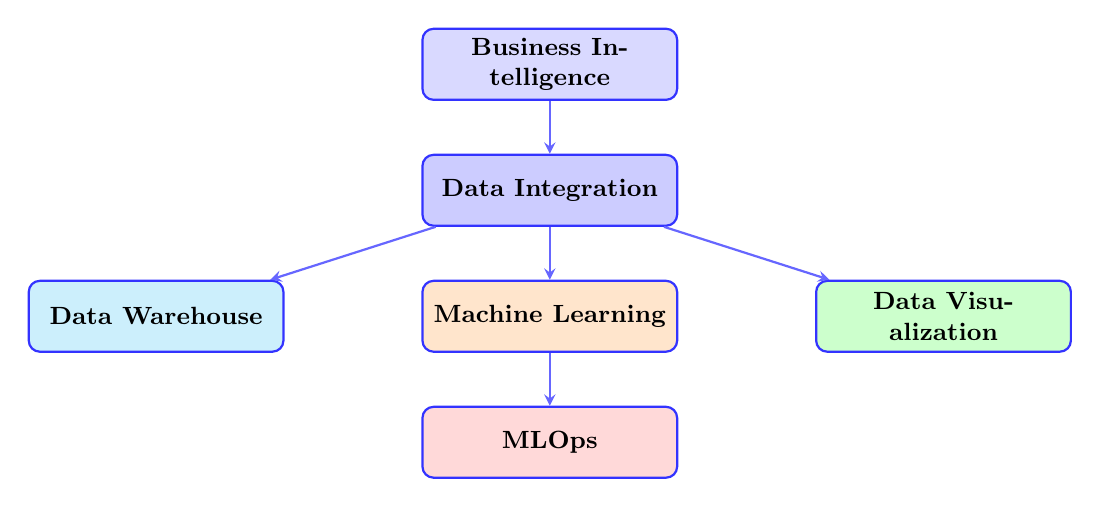
\begin{tikzpicture}[
    box/.style={rectangle, draw=blue!80, thick, fill=blue!10, text width=3.0cm,
    align=center, minimum height=0.9cm, rounded corners=4pt, font=\small\bfseries},
    arrow/.style={->, thick, blue!60, >=stealth}
]
\node[box, fill=blue!15] (bi) at (0,0) {Business Intelligence};
\node[box, fill=blue!20] (integration) at (0,-1.6) {Data Integration};
\node[box, fill=cyan!20] (dwh) at (-5.0,-3.2) {Data Warehouse};
\node[box, fill=orange!20] (ml) at (0,-3.2) {Machine Learning};
\node[box, fill=green!20] (viz) at (5.0,-3.2) {Data Visualization};
\node[box, fill=red!15] (mlops) at (0,-4.8) {MLOps};

\draw[arrow] (bi) -- (integration);
\draw[arrow] (integration) -- (dwh);
\draw[arrow] (integration) -- (ml);
\draw[arrow] (integration) -- (viz);
\draw[arrow] (ml) -- (mlops);
\end{tikzpicture}
\caption{Hierarchy of analytical domains in a Business Intelligence system\cite{chaudhuri2011}}
\label{fig:bi_domain_hierarchy}
\end{figure}
\FloatBarrier
\FloatBarrier

%----------------------------------------------
\subsection{Business Intelligence for Banking}
%----------------------------------------------

Banks rely on BI systems to monitor customer behaviour, detect risk exposure, analyse
commercial performance, and support regulatory compliance \cite{bcbs2011}. Unlike generic
dashboards, banking BI must handle sensitive customer information, account-level financial
metrics, compliance indicators, and traceable risk calculations that can be audited by
internal control teams.

According to the Basel Committee on Banking Supervision \cite{bcbs2011}, effective banking
supervision requires institutions to maintain consolidated, accurate, and timely data on
their customer base, credit exposures, and compliance posture. BI platforms directly address
this requirement by providing governed, auditable analytical pipelines.

In the ATB project, the banking context is represented by two major analytical domains:

\begin{itemize}
    \item \textbf{Customer portfolio analytics}: customer distribution by gender, employment
    status, nationality, sector, industry, target segment, branch, account count, balances,
    and overdraft activity.
    \item \textbf{Customer risk and compliance analytics}: KYC completeness, PEP status,
    compliance flags, posting restrictions, account behaviour, salary availability, dependent
    load, and composite risk scoring \cite{fatf2012}.
\end{itemize}

The ATB project therefore transforms raw operational banking records into a decision-support
platform covering three levels of analysis: descriptive (portfolio dashboards), risk and
compliance (KYC, PEP, scoring), and predictive (ML risk classification).

%----------------------------------------------
\subsection{Machine Learning: Definitions and Learning Paradigms}
%----------------------------------------------

\subsubsection{Definition and Learning Paradigms}

Machine Learning (ML), defined by Mitchell \cite{mitchell1997}, enables computers to learn
from data without being explicitly programmed for each task. Rather than following hard-coded
rules, a machine learning system \textit{generalises} patterns observed in training data and
applies them to new, unseen examples. Mitchell's formal definition states:
\textit{``A computer program is said to learn from experience E with respect to some class of
tasks T and performance measure P, if its performance at tasks in T, as measured by P,
improves with experience E.''} \cite{mitchell1997}

The scientific literature distinguishes three main learning paradigms
\cite{hastie2009, bishop2006}. Table~\ref{tab:ml_paradigms_general} presents these three
paradigms.

\begin{table}[H]
\centering
\small
\caption{The three paradigms of machine learning}
\label{tab:ml_paradigms_general}
\begin{tabular}{|p{3.5cm}|p{4.5cm}|p{4.5cm}|}
\hline
\rowcolor{blue!15}
\textbf{Paradigm} & \textbf{Principle} & \textbf{Typical application} \\
\hline
\textbf{Supervised learning} & Learns from labelled examples
(input $\to$ known output) & Classification, regression, risk scoring \\
\hline
\textbf{Unsupervised learning} & Discovers hidden structures in
unlabelled data & Clustering, dimensionality reduction, anomaly detection \\
\hline
\textbf{Reinforcement learning} & Learns by trial-and-error interaction
with an environment & Robotics, game-playing, sequential optimisation \\
\hline
\end{tabular}
\end{table}

\subsubsection{Supervised Learning}

In supervised learning, the algorithm is trained on a dataset containing both input
variables and the expected outputs (labels). The objective is to learn a function
$f: X \to y$ that maps each input to its corresponding output, so that the model can
accurately predict the label of previously unseen data \cite{mitchell1997}. Bishop
\cite{bishop2006} distinguishes two types of supervised problems: \textbf{classification},
which predicts a discrete label (e.g., fraud / non-fraud, high risk / low risk), and
\textbf{regression}, which predicts a continuous numerical value (e.g., credit amount, churn
probability). The quality of a supervised model is measured by comparing its predictions
against a held-out test set, using metrics such as accuracy, precision, recall, F1-score,
and ROC-AUC.

Among the most effective supervised algorithms for structured tabular data are
\textbf{ensemble methods}: Random Forest \cite{breiman2001}, which combines multiple
decision trees through bagging, and \textbf{XGBoost} \cite{chen2016}, which uses gradient
boosting to sequentially correct the errors of previous trees. These two families have
dominated classification benchmarks in the scientific literature for over a decade
\cite{lessmann2015, baesens2003}.

\subsubsection{Unsupervised Learning}

Unsupervised learning processes unlabelled data to discover latent structures, groupings,
or relationships that are not explicitly encoded in the dataset. The goal is not to predict
a target variable but to understand the underlying organisation of the data
\cite{hastie2009}. Common techniques include:

\begin{itemize}
    \item \textbf{Clustering} (e.g., k-means, DBSCAN): groups observations into clusters
    of similar individuals based on their features.
    \item \textbf{Dimensionality reduction} (e.g., PCA, t-SNE): projects high-dimensional
    data into a lower-dimensional representation while preserving essential structure.
    \item \textbf{Anomaly detection}: identifies data points that deviate significantly from
    the learned normal distribution, used in fraud detection and operational monitoring.
\end{itemize}

Hastie et al.\ \cite{hastie2009} emphasise the utility of unsupervised methods for
exploratory data analysis, hypothesis generation, and pre-processing before supervised
model training. Although labels are absent, these techniques provide valuable insights
into data distributions and feature relationships.

\subsubsection{Reinforcement Learning}

Reinforcement learning (RL) involves an agent that interacts with a dynamic environment.
At each step, the agent takes an action, receives a reward or penalty, and updates its
policy to maximise cumulative reward over time \cite{hastie2009}. Unlike supervised
learning, RL does not require a labelled dataset; it learns from the consequences of its
own decisions. Well-known applications include game-playing agents (AlphaGo), robotics, and
dynamic pricing optimisation. However, RL requires a simulation environment and is
particularly suited to sequential decision-making problems where historical tabular data
alone is insufficient.

\begin{figure}[H]
\centering
\begin{tikzpicture}[
    node distance=0.8cm,
    box/.style={rectangle, draw=blue!70, thick, fill=blue!10, text width=4cm,
    text centered, minimum height=0.7cm, rounded corners=2pt, font=\small}
]
\node[box] (ml) {Machine Learning (ML)};
\node[box, below left=1cm and 1cm of ml, fill=green!10] (supervise) {Supervised Learning};
\node[box, below=1cm of ml, fill=orange!10] (non_supervise) {Unsupervised Learning};
\node[box, below right=1cm and 1cm of ml, fill=red!10] (renforcement) {Reinforcement Learning};
\draw[->, thick, blue!50] (ml) -- (supervise);
\draw[->, thick, blue!50] (ml) -- (non_supervise);
\draw[->, thick, blue!50] (ml) -- (renforcement);
\end{tikzpicture}
\caption{The three machine learning paradigms \cite{mitchell1997, hastie2009}}
\label{fig:ml_paradigms_fig}
\end{figure}

%----------------------------------------------
\subsection{Machine Learning for Banking}
%----------------------------------------------

The banking sector is one of the most data-rich domains and among the earliest adopters of
machine learning. Banks accumulate vast amounts of structured data: customer demographics,
account transaction histories, credit balances, behavioural indicators, and regulatory
attributes. This data richness makes banking a particularly fertile ground for supervised ML
applications \cite{hand1997}.

\subsubsection{(1)Principal Applications of ML in Banking}

Table~\ref{tab:ml_banking_applications} summarises the main application domains of machine
learning in the banking sector.

\begin{table}[H]
\centering
\small
\caption{Principal machine learning applications in banking}
\label{tab:ml_banking_applications}
\begin{tabular}{|p{4cm}|p{8cm}|}
\hline
\rowcolor{blue!15}
\textbf{Application domain} & \textbf{Description} \\
\hline
Credit scoring & Predicts the probability of default for loan applicants using financial
and behavioural features \cite{hand1997, lessmann2015}. \\
\hline
Fraud detection & Identifies anomalous transactions in real time using classification and
anomaly detection models \cite{breiman2001}. \\
\hline
Customer risk profiling & Segments customers by risk level based on compliance, financial
fragility, and behavioural signals \cite{baesens2003}. \\
\hline
Churn prediction & Anticipates customers likely to close accounts or reduce activity,
enabling proactive retention \cite{hastie2009}. \\
\hline
AML / KYC compliance & Flags suspicious transactions and incomplete customer due diligence
as required by FATF recommendations \cite{fatf2012}. \\
\hline
Portfolio analytics & Segments the customer portfolio by risk, sector, and behaviour to
support strategic decision-making \cite{bcbs2011}. \\
\hline
\end{tabular}
\end{table}

\subsubsection{(2)Supervised Models in Banking: Ensemble Methods}

Among the families of supervised algorithms, tree-based ensemble methods have established
themselves as the most reliable for structured banking data. Breiman's \textbf{Random
Forest} \cite{breiman2001} combines a large number of decision trees trained on bootstrap
samples of the data. By averaging their predictions, it reduces variance and achieves robust
generalisation even on noisy datasets. Its feature importance mechanism makes it inherently
interpretable at the variable level, which is essential in regulated environments.

\textbf{XGBoost} (eXtreme Gradient Boosting), introduced by Chen and Guestrin
\cite{chen2016}, builds trees iteratively where each new tree corrects the residual errors
of the previous ensemble. It introduces several regularisation mechanisms (L1 and L2
penalties on tree weights), handles sparse and missing data natively, and supports parallel
computation. Its superior performance on classification benchmarks across structured datasets
has made it the dominant algorithm in financial ML competitions and research publications
\cite{lessmann2015}.

\textbf{Model explainability: SHAP values}

In banking and regulatory contexts, a model must not only be accurate but also
\textit{explainable}. Lundberg and Lee \cite{lundberg2017} introduced SHAP (SHapley
Additive exPlanations), a game-theory-based framework that assigns to each feature a
contribution value for a specific prediction. SHAP values satisfy three desirable
properties: local accuracy (the sum of SHAP values equals the model's output),
missingness (features with value zero receive zero attribution), and consistency.
Their use in banking allows compliance teams to audit individual risk predictions and
verify that model outputs are driven by legitimate business features rather than
spurious correlations.

%----------------------------------------------
\subsection{Machine Learning and Banking Risk Prediction}
%----------------------------------------------

Banking risk prediction is a mature research field that combines statistical scoring,
financial analysis, customer behaviour modelling, and machine learning
\cite{hand1997, bravo2013}. The scientific literature provides strong empirical grounding
for the key design choices of automated risk scoring systems.

\subsubsection{(1)Foundational Works}

Hand and Henley \cite{hand1997} provide a landmark review of statistical classification
methods in consumer credit scoring, establishing that behavioural indicators---account
tenure, payment history, and activity patterns---are complementary to pure financial ratios
and significantly improve default prediction. Their work establishes the multi-signal
approach to risk assessment that has informed all subsequent credit scoring research.

Baesens et al.\ \cite{baesens2003}, in a large-scale benchmark across eight classification
algorithms on real banking datasets, demonstrate that ensemble methods (neural networks,
SVM, and ensemble trees) systematically outperform logistic regression on imbalanced risk
data. This study is a foundational reference justifying the use of tree-based classifiers
over simpler linear baselines in banking applications.

Lessmann et al.\ \cite{lessmann2015} extend this benchmark with more modern algorithms and
18 real-world credit datasets, confirming that gradient-boosted ensembles and random forests
consistently rank at the top for structured financial data. They also demonstrate that
accuracy alone is an insufficient evaluation metric under class imbalance and recommend
the F1-score, ROC-AUC, and PR-AUC as the primary evaluation criteria.

Dastile et al.\ \cite{dastile2020} conduct a systematic literature survey of credit scoring
models from 2000 to 2020, identifying three recurring challenges: (1)~class imbalance
between defaulters and non-defaulters; (2)~temporal instability of scoring models requiring
regular retraining; and (3)~the growing regulatory requirement for interpretable ML
predictions. They confirm that XGBoost and Random Forest dominate recent production
deployments.

Bravo et al.\ \cite{bravo2013} identify structural challenges specific to banking credit
scoring: data scarcity for rare risk events, selection bias in historical data, and the
need for reject inference when the approval process filters the training population. These
findings motivate the use of resampling techniques such as SMOTETomek to address class
imbalance, and held-out evaluation designs that prevent target leakage.

\subsubsection{(2)Regulatory Risk Drivers}

From a regulatory perspective, the FATF Recommendations \cite{fatf2012} establish that
incomplete Know Your Customer (KYC) data, Politically Exposed Person (PEP) exposure, and
compliance flags must be treated as \textit{primary} risk signals, preceding any financial
analysis. The Basel Committee on Banking Supervision \cite{bcbs2011} further formalises the
principle of multi-pillar risk assessment: compliance, financial, and behavioural dimensions
must be combined into a single, auditable, supervised risk view. This regulatory framework
directly justifies a weighted composite risk score combining three pillars:
\begin{equation}
\label{eq:global_risk_score}
\mathrm{GRS} = 0.40\,\mathrm{CRI} + 0.35\,\mathrm{FFS} + 0.25\,\mathrm{BRS},
\end{equation}
where $\mathrm{CRI}$, $\mathrm{FFS}$, and $\mathrm{BRS}$ denote respectively the
Compliance Risk Index, Financial Fragility Score, and Behavioural Risk Score, each
scaled to $[0,100]$.

\subsubsection{(3)Tree-Based Models for Risk Classification}

Based on the above literature, two tree-based ensemble models are retained and compared
for customer risk classification:

\begin{table}[H]
\centering
\small
\caption{Comparative justification of the ML models used for banking risk prediction}
\label{tab:atb_ml_models}
\begin{tabular}{|p{3cm}|p{5cm}|p{5.2cm}|}
\hline
\rowcolor{blue!15}
\textbf{Model} & \textbf{Properties} & \textbf{Scientific justification} \\
\hline
\textbf{Random Forest} \cite{breiman2001} &
Bagging ensemble; low variance; stable feature importance; resistant to overfitting. &
Robust baseline for tabular banking data; validated by Baesens et al.\ \cite{baesens2003}
and Lessmann et al.\ \cite{lessmann2015}. \\
\hline
\textbf{XGBoost} \cite{chen2016} &
Gradient boosting; handles imbalance; L1/L2 regularisation; fast and parallelisable. &
Top performer across credit scoring benchmarks \cite{lessmann2015, dastile2020}; handles
sparse banking features efficiently. \\
\hline
\end{tabular}
\end{table}




%----------------------------------------------
\subsection{Evaluation Metrics for Predictive Banking Systems}
%----------------------------------------------

The evaluation of a banking risk classifier must consider both classification performance
and probability quality. In an imbalanced risk problem, accuracy alone is insufficient
because a model may achieve high accuracy simply by predicting the majority class
\cite{lessmann2015}. The following complementary metrics are used:

\begin{table}[H]
\centering
\caption{Evaluation metrics for the ATB customer risk classifier}
\label{tab:atb_ml_metrics}
\begin{tabular}{|p{3cm}|p{5.5cm}|p{4.2cm}|}
\hline
\rowcolor{blue!15}
\textbf{Metric} & \textbf{Definition} & \textbf{Purpose} \\
\hline
Accuracy & Proportion of correct predictions. & Global performance indicator. \\
\hline
Precision & Share of predicted high-risk customers that are truly high risk. &
Limits false alerts. \\
\hline
Recall & Share of true high-risk customers detected by the model. &
Limits missed risky customers. \\
\hline
F1-score & Harmonic mean of precision and recall. &
Main selection metric for imbalanced classes. \\
\hline
ROC-AUC & Ability to rank positive cases above negative cases. &
Threshold-independent discrimination. \\
\hline
PR-AUC & Area under the precision-recall curve. &
More informative under class imbalance. \\
\hline
Brier score & Mean squared error of predicted probabilities. &
Probability calibration quality. \\
\hline
\end{tabular}
\caption*{\small Standard metrics in credit scoring and banking ML benchmarking
\cite{lessmann2015, hand1997}}
\end{table}

On the held-out test set, the ATB model selection notebook reports the following results:

\begin{itemize}
    \item \textbf{XGBoost (selected model)}: Accuracy = 99.8\%, F1 = 94.5\%,
    Precision = 96.3\%, Recall = 92.9\%, ROC-AUC = 0.998, PR-AUC = 0.953.
    \item \textbf{Random Forest (benchmark)}: Accuracy = 99.6\%, F1 = 88.0\%,
    Precision = 100.0\%, Recall = 78.6\%, ROC-AUC = 0.994, PR-AUC = 0.953.
\end{itemize}

XGBoost is promoted to Production in MLflow because it outperforms Random Forest on F1,
recall, and ROC-AUC while maintaining an acceptable generalisation gap.


%================================================
\section{Data Engineering for Decision-Support Systems}
%================================================

%----------------------------------------------
\subsection{Architecture of a Decision-Support System}
%----------------------------------------------

According to Chaudhuri and Dayal \cite{chaudhuri2011}, a decision-support system generally
includes data sources, integration, staging, warehouse modelling, analytics, and
presentation layers. This architecture is the standard reference model for BI platforms.

\begin{figure}[H]
\centering
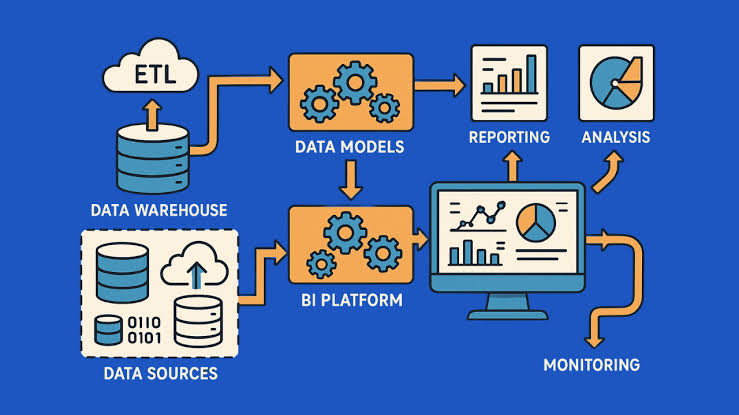
\includegraphics[width=0.6\textwidth]{architecture_bi.png}
\caption{Architecture of a Business Intelligence system \cite{chaudhuri2011}}
\label{fig:architecture_bi_atb}
\end{figure}

The detailed structure of such a system comprises the following elements:

\begin{itemize}
    \item \textbf{Data sources}: heterogeneous operational data generated inside and outside
    the organisation.
    \item \textbf{ETL/ELT process}: extracts, optionally transforms, and loads data into a
    centralised repository.
    \item \textbf{Operational Data Store (ODS)}: intermediate staging area between operational
    sources and the data warehouse.
    \item \textbf{Data Warehouse}: centralised database organising structured data for
    analytical queries.
    \item \textbf{Data Marts}: domain-specific subsets of the warehouse.
    \item \textbf{Analytical layer}: OLAP cubes, ML models, and reporting tools.
    \item \textbf{Visualisation}: dashboards and reports for business decision-makers.
\end{itemize}


%----------------------------------------------
\subsection{ETL and ELT Paradigms}
%----------------------------------------------

Data integration is the backbone of any decision-support system. Rahm and Do \cite{rahm2000}
formalise the data quality challenges encountered during extraction, transformation, and
loading: schema heterogeneity, null handling, encoding inconsistencies, and duplicate
records. Two main integration paradigms exist:

\begin{table}[H]
\centering
\caption{Comparative analysis of ETL versus ELT}
\label{tab:atb_etl_elt}
\begin{tabular}{|p{3cm}|p{5cm}|p{5cm}|}
\hline
\rowcolor{blue!15}
\textbf{Aspect} & \textbf{ETL} & \textbf{ELT} \\
\hline
Maturity & Mature, widely adopted & Emerging cloud-native pattern \\
\hline
Data type & Structured operational data & Structured and semi-structured data \\
\hline
Transformation location & Outside the warehouse & Inside the database engine \\
\hline
Traceability & External transformation scripts & Versioned SQL models (e.g., dbt) \\
\hline
Typical use & Traditional BI, on-premise DWH & Data Lakes, Cloud, modern DWH \\
\hline
\end{tabular}
\end{table}

The ATB project follows an \textbf{ELT-oriented architecture}: data from seven
pipe-separated CSV files is first loaded into the SQL Server ODS schema
(\texttt{PFE\_ODS}), then transformed using versioned dbt SQL models inside the database.
This choice aligns with Kimball's recommendation \cite{kimball2013} to perform
transformations as close to the analytical store as possible, enabling full lineage tracking
and reproducibility.

The transformation layer is divided into three levels:

\begin{itemize}
    \item \textbf{Staging}: cleans raw ODS data, casts types, standardises names,
    and preserves source truth.
    \item \textbf{Intermediate}: applies business logic, joins reference data, computes
    account aggregates, and calculates the three-pillar risk scores.
    \item \textbf{Warehouse}: builds conformed dimensions and fact tables for BI, ML,
    and reporting.
\end{itemize}

%----------------------------------------------
\subsection{Data Warehouse, Data Lake, and Data Mart}
%----------------------------------------------

The choice of the appropriate data storage paradigm is a critical architectural decision in
any decision-support system. Three complementary concepts are defined in the literature:
the Data Warehouse, the Data Lake, and the Data Mart. Understanding their differences allows
an informed selection based on the nature of the data, the analytical requirements, and the
technical maturity of the organisation \cite{kimball2013, inmon2005}.

\textbf{(1) Data Warehouse (DWH)}

A Data Warehouse (DWH) is a centralised, subject-oriented, integrated, non-volatile, and
time-variant data repository designed to support analytical queries and decision-making at
the enterprise level \cite{inmon2005}. Inmon's definition emphasises four key properties:

\begin{itemize}
    \item \textbf{Subject-oriented}: organised around business subjects (customers, accounts,
    risk) rather than operational transactions.
    \item \textbf{Integrated}: data from heterogeneous sources is harmonised into a single
    consistent schema.
    \item \textbf{Non-volatile}: once written, records are not modified or deleted; history
    is preserved.
    \item \textbf{Time-variant}: each record carries a temporal reference, enabling
    historical analysis and trend monitoring.
\end{itemize}

Kimball \cite{kimball2013} extends this definition by proposing the dimensional modelling
approach: data is organised around fact tables (quantitative measurements) and dimension
tables (analytical context), forming star, snowflake, or constellation schemas optimised
for analytical query performance.

\textbf{(2) Data Lake}

A Data Lake is a large-scale, schema-on-read storage repository that ingests raw data in
its original format---structured, semi-structured, or unstructured---and defers the
application of structure until query time \cite{kimball2013}. Unlike a Data Warehouse, a
Data Lake does not impose a predefined schema on ingestion, making it flexible for storing
diverse data types (logs, JSON, images, streams). However, without governance, a Data Lake
can degrade into a ``Data Swamp'' where data is stored but not usable.

The key differences between a Data Lake and a Data Warehouse are:

\begin{itemize}
    \item \textbf{Schema}: schema-on-read (Data Lake) versus schema-on-write (Data Warehouse).
    \item \textbf{Data type}: any format (Data Lake) versus structured only (Data Warehouse).
    \item \textbf{Target user}: data scientists exploring raw data (Data Lake) versus
    business analysts querying governed KPIs (Data Warehouse).
    \item \textbf{Performance}: flexible but slower for aggregated queries (Data Lake) versus
    optimised for analytical workloads (Data Warehouse).
\end{itemize}

\textbf{(3) Data Mart}

A Data Mart is a domain-specific, scoped subset of a Data Warehouse, tailored to the
analytical needs of a specific business unit or subject area \cite{inmon2005}. It is smaller
than a full enterprise warehouse and faster to query for its focused domain. Data Marts
can be dependent (derived from a central DWH) or independent. The bottom-up Kimball
approach builds the enterprise warehouse progressively through interconnected Data Marts
sharing conformed dimensions.

\begin{table}[H]
\centering
\small
\renewcommand{\arraystretch}{1.4}
\caption{Comparison: Data Warehouse, Data Lake, and Data Mart}
\label{tab:dwh_lake_mart}
\begin{tabular}{|p{3cm}|p{3.7cm}|p{3.7cm}|p{3.7cm}|}
\hline
\rowcolor{blue!15}
\textbf{Criterion} & \textbf{Data Warehouse} & \textbf{Data Lake} & \textbf{Data Mart} \\
\hline
Data type & Structured, governed & Any (raw, unstructured) & Structured, domain-scoped \\
\hline
Schema & Schema-on-write & Schema-on-read & Schema-on-write \\
\hline
Scope & Enterprise-wide & Organisation-wide & Business unit or subject \\
\hline
Users & Business analysts, BI tools & Data scientists, engineers & Domain analysts \\
\hline
Query performance & High (optimised) & Lower (flexible) & Very high (focused) \\
\hline
Complexity & High & Medium (governance risk) & Low \\
\hline
Example technology & SQL Server, Oracle DWH & AWS S3, Azure Data Lake & PostgreSQL subject mart \\
\hline
\end{tabular}
\end{table}

%----------------------------------------------
\subsection{Multidimensional Modelling}
%----------------------------------------------

In multidimensional modelling, a schema is composed of a central \textbf{fact table} and
\textbf{dimension tables} \cite{kimball2013}. Three standard schema types are defined in
the literature:

\textbf{(1) Star Schema}

A star schema contains one central fact table surrounded by denormalised dimensions,
forming a structure resembling a star. It is simple and performant for BI dashboards.

\begin{figure}[H]
\centering
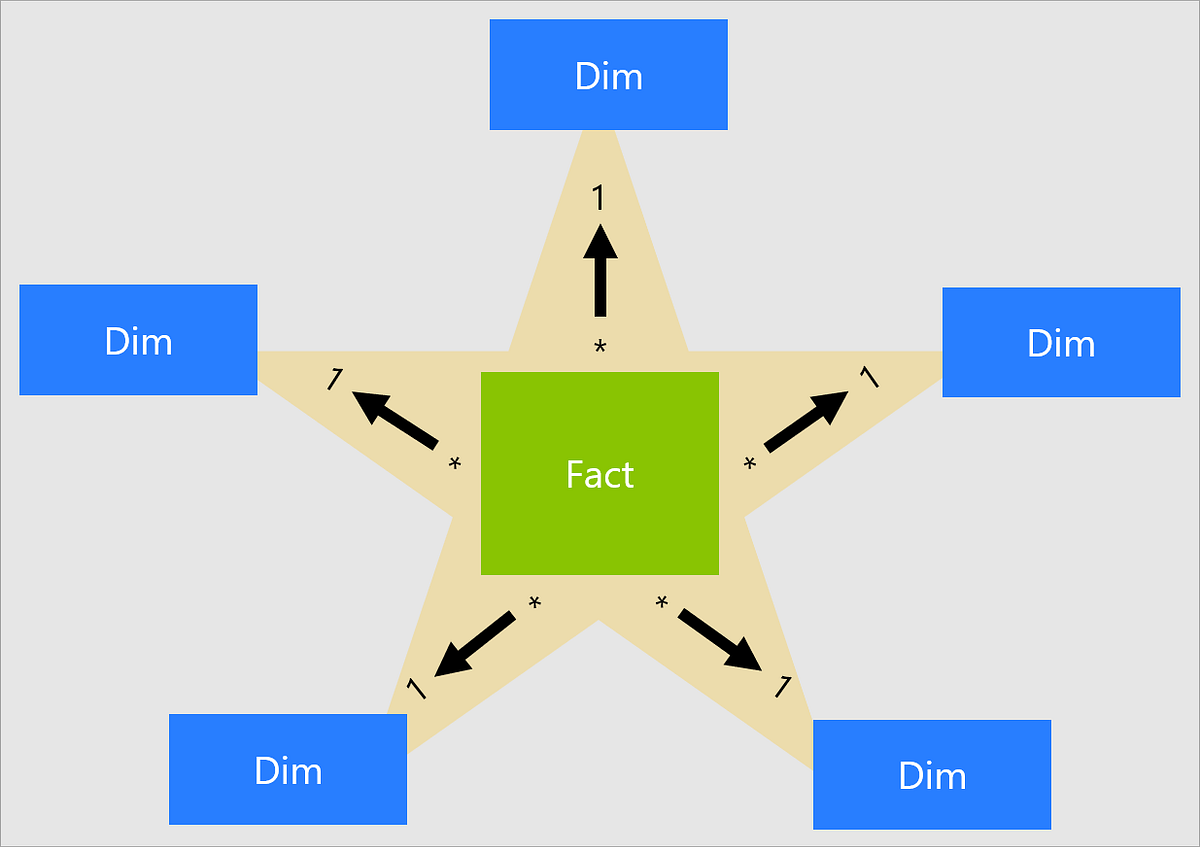
\includegraphics[width=0.4\textwidth]{star_schema.png}
\caption{Star schema dimensional modelling \cite{kimball2013}}
\label{fig:star_schema_atb}
\end{figure}

\textbf{(2) Snowflake Schema}

A snowflake schema normalises dimension tables into subdimensions. It can reduce redundancy
but increases join complexity \cite{inmon2005}.

\begin{figure}[H]
\centering
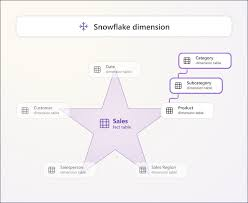
\includegraphics[width=0.4\textwidth]{snowflake_schema.png}
\caption{Snowflake schema dimensional modelling \cite{inmon2005}}
\label{fig:snowflake_schema_atb}
\end{figure}

\textbf{(3) Constellation Schema (Galaxy Schema)}

A constellation schema contains several fact tables sharing conformed dimensions. This is
the \textbf{selected model} for the ATB project, as it supports both account-level analytics
and customer risk analytics through two independent fact tables that share common dimensions
\cite{kimball2013}.

\begin{figure}[H]
\centering
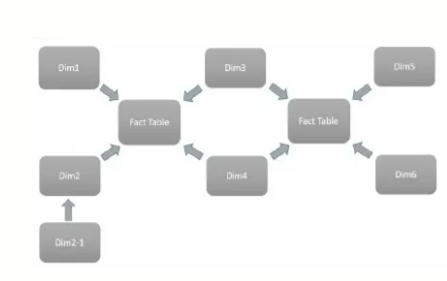
\includegraphics[width=0.5\textwidth]{galaxy_schema.png}
\caption{Constellation (galaxy) schema dimensional modelling \cite{kimball2013}}
\label{fig:galaxy_schema_atb}
\end{figure}

\begin{table}[H]
\centering
\small
\caption{ATB constellation warehouse structure}
\label{tab:atb_constellation}
\begin{tabular}{|p{4cm}|p{4.5cm}|p{5cm}|}
\hline
\rowcolor{blue!15}
\textbf{Component} & \textbf{Grain} & \textbf{Purpose} \\
\hline
\textbf{fact\_account} & One row per account snapshot & Descriptive analytics: balance,
overdraft flag, credit balance, account age. \\
\hline
\textbf{fact\_customer\_risk} & One row per customer per scoring date & Risk analytics:
CRI, FFS, BRS, global risk score, risk tier. \\
\hline
\textbf{Shared dimensions} & Customer, DAO, sector, industry, target, date & Common
analytical context for both facts. \\
\hline
\textbf{Specific dimensions} & Currency, risk profile & Currency (accounts); risk profile
(customer risk). \\
\hline
\end{tabular}
\end{table}

The ATB warehouse contains 8 dimensions and 2 fact tables (281,960 total rows,
0 null foreign keys).

%----------------------------------------------
\subsection{Data Warehouse Design Approaches}
%----------------------------------------------

\textbf{(1) Bottom-Up Approach (Kimball)}

Initiated by Ralph Kimball \cite{kimball2013}, this approach builds the warehouse
progressively through dimensional data marts connected by conformed dimensions. It is
particularly suited to BI projects requiring early dashboard delivery and business-readable
models.

\begin{figure}[H]
\centering
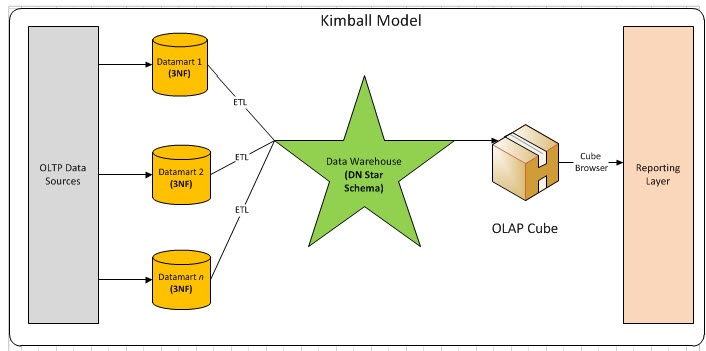
\includegraphics[width=0.65\textwidth]{kimball_model.png}
\caption{Bottom-up approach according to Ralph Kimball \cite{kimball2013}}
\label{fig:kimball_atb}
\end{figure}

The ATB project follows a Kimball-oriented approach: conformed dimensions are built first,
then fact tables for account analytics and customer risk analytics.

\textbf{(2) Top-Down Approach (Inmon)}

Initiated by Bill Inmon \cite{inmon2005}, this approach begins with a centralised enterprise
data warehouse before deriving specialised data marts. It requires more upfront modelling
effort but maintains stronger enterprise-level consistency.

\begin{figure}[H]
\centering
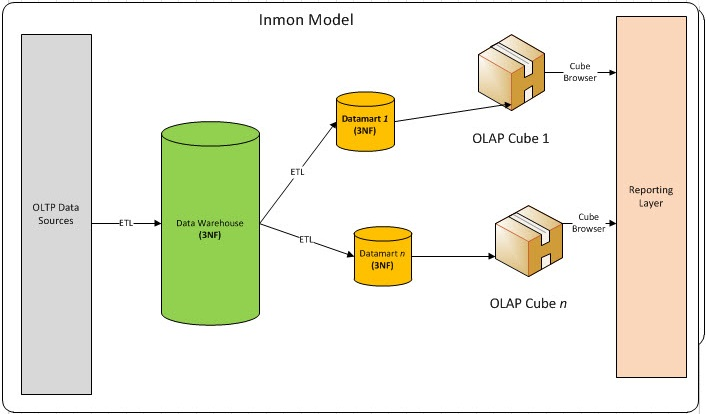
\includegraphics[width=0.65\textwidth]{inmon_model.png}
\caption{Top-down approach according to Bill Inmon \cite{inmon2005}}
\label{fig:inmon_atb}
\end{figure}

\textbf{(3) Hybrid Approach}

A hybrid approach combines enterprise consistency with incremental delivery
\cite{kimball2013, inmon2005}. The ATB project can be considered hybrid in practice
because it uses a central SQL Server warehouse while delivering domain-focused facts for
account analytics and risk analytics independently.

\begin{figure}[H]
\centering
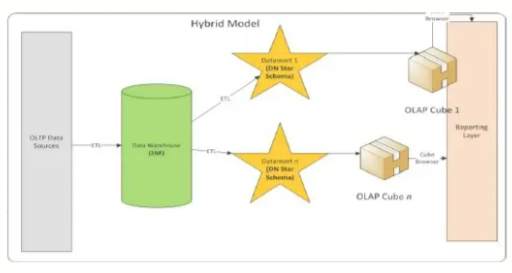
\includegraphics[width=0.65\textwidth]{hybrid_model.png}
\caption{Hybrid data warehouse approach (Inmon + Kimball) \cite{kimball2013, inmon2005}}
\label{fig:hybrid_atb}
\end{figure}

%----------------------------------------------
\subsection{Key Performance Indicators (KPI)}
%----------------------------------------------

KPIs constitute the common language between technical data processing and business
decision-making. According to Eckerson \cite{eckerson2010}, a good BI dashboard must
integrate three types of indicators:

\begin{itemize}
    \item \textbf{Strategic KPIs}: global view of portfolio and risk performance.
    \item \textbf{Operational KPIs}: daily monitoring of accounts, compliance alerts, and
    branch activity.
    \item \textbf{Leading KPIs}: predictive signals from ML scores and drift monitoring.
\end{itemize}

\begin{table}[H]
\centering
\small
\caption{Main KPI families of the ATB BI platform}
\label{tab:atb_kpis}
\begin{tabular}{|p{4cm}|p{5cm}|p{4.2cm}|}
\hline
\rowcolor{blue!15}
\textbf{KPI family} & \textbf{Examples} & \textbf{Business value} \\
\hline
Customer portfolio & Total customers, distribution by employment, sector, gender, branch. &
Understand the structure of the customer base. \\
\hline
Account analytics & Total accounts, total working balance, average balance, overdraft rate,
account age. & Monitor financial portfolio health. \\
\hline
Risk and compliance & Global risk score, risk tier distribution, KYC completeness, PEP count,
compliance flags. & Prioritise controls and compliance actions. \\
\hline
ML performance & Accuracy, F1-score, ROC-AUC, PR-AUC, Brier score. &
Monitor model quality and predictive reliability. \\
\hline
Data quality & Row counts, null foreign keys, referential integrity, freshness timestamps. &
Guarantee trustworthy dashboard outputs. \\
\hline
\end{tabular}
\end{table}

%----------------------------------------------
\subsection{Foundational Works on Banking Risk Scoring}
%----------------------------------------------

The ATB composite risk score is grounded in four foundational references from the
scientific literature:

\textbf{(1) Regulatory compliance as a first-order risk driver.}
The FATF Recommendations \cite{fatf2012} establish that incomplete KYC data, PEP exposure,
and compliance flags must be treated as primary risk signals before any financial analysis.
This justifies dedicating the highest pillar weight (40\%) to the Compliance Risk Index.

\textbf{(2) Financial fragility as a credit-scoring predictor.}
Lessmann et al.\ \cite{lessmann2015} demonstrate through a large-scale classification
benchmark that financial variables---salary, balance levels, and overdraft behaviour---are
the strongest predictors of financial vulnerability. This supports the Financial Fragility
Score as the second pillar (35\%).

\textbf{(3) Behavioural patterns as complementary signals.}
Hand and Henley \cite{hand1997} show that consumer credit scoring benefits from behavioural
indicators (account tenure, payment history, activity patterns) complementing pure financial
ratios. The Behavioural Risk Score (25\%) captures customer tenure, negative balances, and
KYC staleness.

\textbf{(4) Multi-pillar aggregation.}
The Basel~III framework \cite{bcbs2011} formalises that bank risk must be assessed through
complementary pillars aggregated into a single supervisory view. Eckerson \cite{eckerson2010}
extends this logic to BI dashboards via weighted composite KPIs.



%================================================
\section{MLOps and Traceability: MLflow}
%================================================

%----------------------------------------------
\subsection{Challenges of Machine Learning in Production}
%----------------------------------------------

Sculley et al.\ \cite{sculley2015} formalised the concept of technical debt in production
ML systems, identifying three structural challenges:

\begin{enumerate}
    \item \textbf{Reproducibility}: a model trained today must be reproducible with the
    same code, data preparation logic, parameters, and random seed.
    \item \textbf{Traceability}: every experiment must preserve its full context
    (parameters, metrics, artefacts, data version).
    \item \textbf{Comparability}: performance across model versions must be directly
    comparable to enable data-driven model selection.
\end{enumerate}

These challenges are amplified in a banking context where model outputs must be
auditable, explainable, and reproducible for regulatory compliance.

%----------------------------------------------
\subsection{MLflow: Architecture and Components}
%----------------------------------------------

MLflow, developed by Databricks \cite{zaharia2018}, has become the reference platform for
managing the machine learning development lifecycle. To justify this choice, a comparative
analysis of the leading MLOps platforms is presented in Table~\ref{tab:mlops-comparison}.

\begin{table}[H]
\centering
\caption{Comparison of main MLOps platforms}
\label{tab:mlops-comparison}
\begin{tabular}{|l|c|c|c|c|}
\hline
\rowcolor{blue!15}
\textbf{Platform} & \textbf{Tracking} & \textbf{Versioning} & \textbf{Deployment} &
\textbf{Open Source} \\
\hline
MLflow & ++ & ++ & + & \checkmark \\
Kubeflow & + & + & ++ & \checkmark \\
Weights \& Biases & +++ & + & + & Freemium \\
Neptune & ++ & + & + & Freemium \\
\hline
\end{tabular}
\caption*{\small Legend: + (basic support), ++ (advanced support), +++ (exceptional support)}
\end{table}

MLflow provides four core components:

\begin{enumerate}
    \item \textbf{MLflow Tracking}: logs runs, hyperparameters, metrics, thresholds, and
    artefacts for experiment comparison.
    \item \textbf{MLflow Projects}: standardises execution environments for reproducibility.
    \item \textbf{MLflow Models}: packages serialised classifiers as versioned artefacts.
    \item \textbf{MLflow Registry}: manages the model lifecycle (Staging, Production,
    Archived) with audit trails.
\end{enumerate}

\begin{figure}[H]
\centering
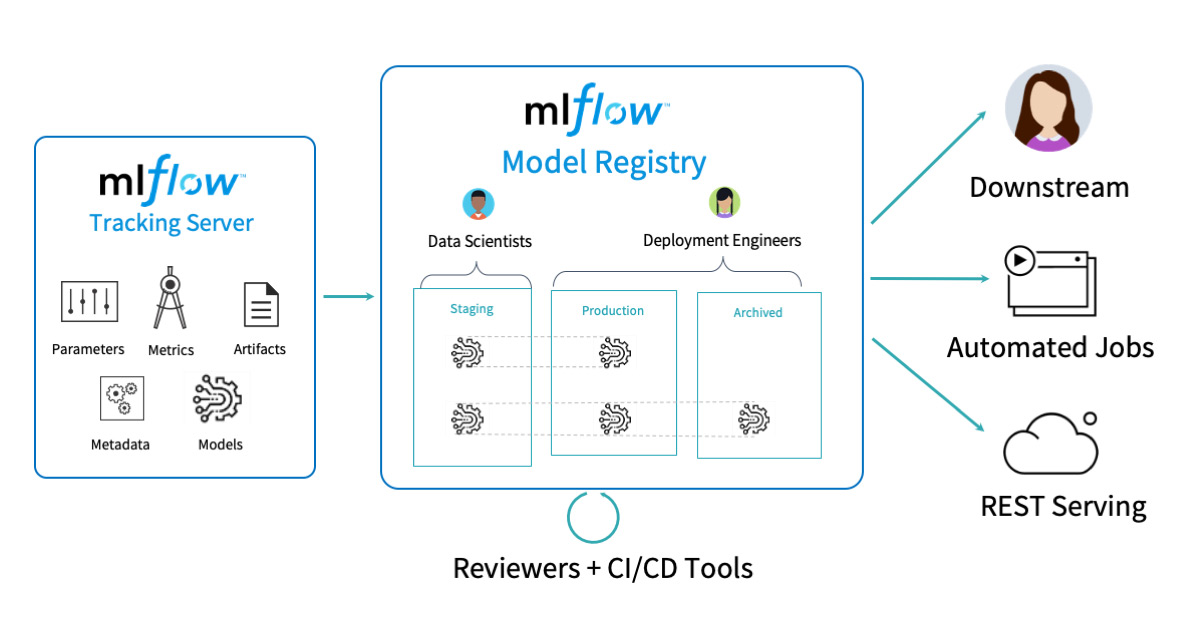
\includegraphics[width=0.8\textwidth]{figures/mlflow_architecture.jpg}
\caption{Architecture de MLflow avec backend SQLite\cite{mlflow_architecture}}
\label{fig:mlflow_architecture}
\end{figure}


%================================================
\section{Generative AI for Dashboard Explanation}
%================================================

%----------------------------------------------
\subsection{Large Language Models (LLMs) in Business Intelligence}
%----------------------------------------------

The emergence of Large Language Models (LLMs) has transformed data interaction paradigms.
In the context of Business Intelligence and analytical reporting, recent studies \cite{baidoo2023}
identify three primary use-cases for LLMs:
\begin{enumerate}
    \item \textbf{Narrative generation}: Translating complex structured reports into accessible text summaries.
    \item \textbf{Intelligent query assistants}: Allowing users to query databases using natural language.
    \item \textbf{Explaining machine learning outputs}: Translating predictions, tree weights, and feature attributions (e.g., SHAP values) into plain corporate language.
\end{enumerate}

%----------------------------------------------
\subsection{Google Gemini for Chart Narration}
%----------------------------------------------

Google Gemini, developed by Google DeepMind \cite{gemini2024}, is a family of multimodal
models optimized for large token contexts, low latency, and advanced reasoning. In this
project, \texttt{gemini-2.0-flash} is used as the sole generative engine for on-demand
chart explanations: a statistical summary of the visible Plotly figure is sent to the
API, which returns a short, role-aware paragraph for banking users.

%----------------------------------------------
\subsection{Availability and Local Template Fallback}
%----------------------------------------------

A practical challenge when calling a commercial LLM API from an operational dashboard is
service availability: rate limits, network issues or a missing API key must not break the
BI application. The ATB platform therefore pairs Gemini with a \textbf{deterministic local
template fallback}: if the API call fails or no key is configured, a pre-authored
explanation sentence is shown instead. This keeps the ``Explain chart'' feature always
usable without introducing a second LLM provider.



%================================================
\section{Data Application Development Frameworks}
%================================================

%----------------------------------------------
\subsection{Streamlit for BI and ML Deployment}
%----------------------------------------------

Bhatt et al.\ \cite{bhatt2021} evaluate the principal Python dashboard frameworks for
data science applications. The ATB project uses Streamlit as the primary operational
dashboard framework, complemented by Jupyter Notebooks for ML development and exploration.

\begin{table}[H]
\centering
\footnotesize
\caption{Comparison of data application frameworks}
\label{tab:atb_reporting_frameworks}
\begin{tabular}{|p{2.8cm}|p{2.4cm}|p{2.4cm}|p{2.4cm}|p{2.4cm}|}
\hline
\rowcolor{blue!15}
\textbf{Criterion} & \textbf{Streamlit} & \textbf{Jupyter} & \textbf{Dash} &
\textbf{Power BI} \\
\hline
Learning curve & Very low & Low & Medium & Medium \\
\hline
ML integration & Excellent & Native & Good & Limited \\
\hline
Role-based pages & In code (RBAC) & Not designed & Custom & Workspace \\
\hline
Banking logic & Full Python & Full Python & Full Python & DAX/M \\
\hline
Interactivity & Native & Via widgets & JavaScript & Native \\
\hline
Project usage & \textbf{Selected} & ML \& EDA & Compared & Compared Ch.~1 \\
\hline
\end{tabular}
\end{table}

The Streamlit dashboard implements role-based navigation for General Management, Chief
Compliance, and Branch Manager profiles, with pages covering executive overview, BI
studies, compliance monitoring, alerts, risk analysis, accounts, MLflow tracking, ML
risk model, and data explorer.


%================================================
\section{Synthesis and Positioning}
%================================================

The state-of-the-art analysis shows that the ATB BI project is positioned at the
intersection of three mature domains: Business Intelligence, data warehousing, and machine
learning. Its scientific added value comes from integrating these domains into a single,
governed, operational banking platform.

Many BI projects stop at descriptive dashboards. Conversely, many ML prototypes remain
disconnected from governed data models and operational reporting. The ATB project addresses
this gap by building a complete, reproducible pipeline: CSV ingestion into SQL Server via
Airbyte and Python, dbt transformations across three layers, a Kimball-style constellation
warehouse with 8 dimensions and 281,960 total rows, Airflow orchestration, MLflow tracking
for full model traceability, SHAP explainability for interpretable audit-grade predictions,
and Streamlit dashboards for banking decision-makers.

The project therefore transforms raw banking data into a governed decision-support platform
capable of descriptive analytics, risk monitoring, predictive classification, and explainable
reporting for ATB stakeholders.


%================================================
\section{Requirements Specification}
%================================================

Requirements specification is a pivotal step in software engineering. It establishes a
clear contract between the banking business needs of the ATB and the technical solution to
be developed, while delimiting the functional scope of the platform.

%----------------------------------------------
\subsection{Actor Identification}
%----------------------------------------------

An actor represents the abstraction of a role played by a human or external system
interacting with the platform. In the ATB system, the following actors have been
identified, each with distinct access rights based on Role-Based Access Control (RBAC):

\begin{itemize}
    \item \textbf{General Management (DG\_CENTRAL)}: accesses executive KPIs, portfolio
    summaries, risk distribution, and high-level monitoring pages.
    \item \textbf{Chief Compliance Officer (CHEF\_CONFORMITE)}: monitors KYC completeness,
    PEP customers, compliance flags, alerts, and customer watchlists.
    \item \textbf{Branch Manager (CHEF\_AGENCE)}: analyses customers and accounts scoped to
    a specific DAO area or branch perimeter.
\end{itemize}

%----------------------------------------------
\subsection{Functional Requirements}
%----------------------------------------------

Functional requirements describe the actions the system must be able to execute in order to
satisfy the business stakeholders. They are categorised by actor role and analytical domain:

\textbf{1. General Management Dashboard Module}
\begin{itemize}
    \item The system must display executive KPI summaries: total customers, total accounts,
    global risk distribution, and portfolio structure.
    \item The system must provide portfolio overview charts by sector, industry, nationality,
    gender, and employment status.
    \item The system must allow export of executive summaries and KPI snapshots to CSV.
    \item The system must display AI-generated plain-language explanations of complex charts.
\end{itemize}

\textbf{2. Compliance and Risk Monitoring Module}
\begin{itemize}
    \item The system must display KYC completeness rates and flag customers with missing
    KYC records.
    \item The system must list PEP customers with associated risk scores and compliance
    alert status.
    \item The system must display risk tier distribution (LOW, MEDIUM, HIGH, VERY\_HIGH)
    with drill-down by branch or DAO area.
    \item The system must provide a compliance alert watchlist with filtering and export
    to CSV.
    \item The system must visualise the three-pillar risk score decomposition (CRI, FFS,
    BRS) per customer or segment.
\end{itemize}

\textbf{3. Branch Analytics Module}
\begin{itemize}
    \item The system must filter all dashboard views to the DAO area or branch scope
    assigned to the Branch Manager.
    \item The system must display account activity metrics: working balance, overdraft rate,
    account age, and credit balance for the managed perimeter.
    \item The system must allow comparison of branch performance against the global
    portfolio benchmark.
    \item The system must provide customer-level drill-down within the managed branch perimeter.
\end{itemize}

\textbf{4. Machine Learning and Predictive Analytics Module}
\begin{itemize}
    \item The system must expose XGBoost risk predictions for all customers in a dedicated
    ML dashboard page.
    \item The system must display SHAP feature importance plots for model interpretability.
    \item The system must provide MLflow experiment tracking data (metrics, parameters,
    artefacts) in a dedicated MLflow page.
    \item The system must allow on-demand batch scoring and write results to the
    \texttt{PFE\_ML} schema.
\end{itemize}

%----------------------------------------------
\subsection{Non-Functional Requirements}
%----------------------------------------------

Non-functional requirements define quality, performance, confidentiality, and maintainability
constraints that the architectural design must satisfy:

\begin{itemize}
    \item \textbf{Data quality}: fact tables must have 0 null foreign keys, valid referential
    integrity, controlled row counts, and freshness timestamps.
    \item \textbf{Performance}: the daily warehouse pipeline must complete within
    approximately 35 minutes, with optional ML retraining triggered as a downstream batch step.
    \item \textbf{Traceability}: dbt models, Airflow DAGs, ML runs, model metrics, and
    artefacts must be versioned and auditable through MLflow.
    \item \textbf{Confidentiality}: access to customer data, risk scores, and compliance
    information must be restricted to authorised roles only through RBAC; data must remain
    within ATB's internal infrastructure.
    \item \textbf{Availability}: the daily pipeline must be monitored with Airflow retry
    mechanisms and alerting to ensure consistent data freshness for morning dashboard sessions.
    \item \textbf{Maintainability}: the project must remain modular through separation of
    the five implementation folders.
    \item \textbf{Explainability}: risk scores must be interpretable through three business
    pillars, and model behaviour must be explained through SHAP artefacts.
    \item \textbf{Usability}: dashboards must provide readable KPIs, clear navigation,
    consistent colours, and business-oriented explanations.
\end{itemize}

%----------------------------------------------
\subsection{Architectural View of Use Cases}
%----------------------------------------------

In order to formalise the interactions between actors and the system, the functional
requirements are modelled through a global use case diagram.
\begin{figure}[H]
\centering
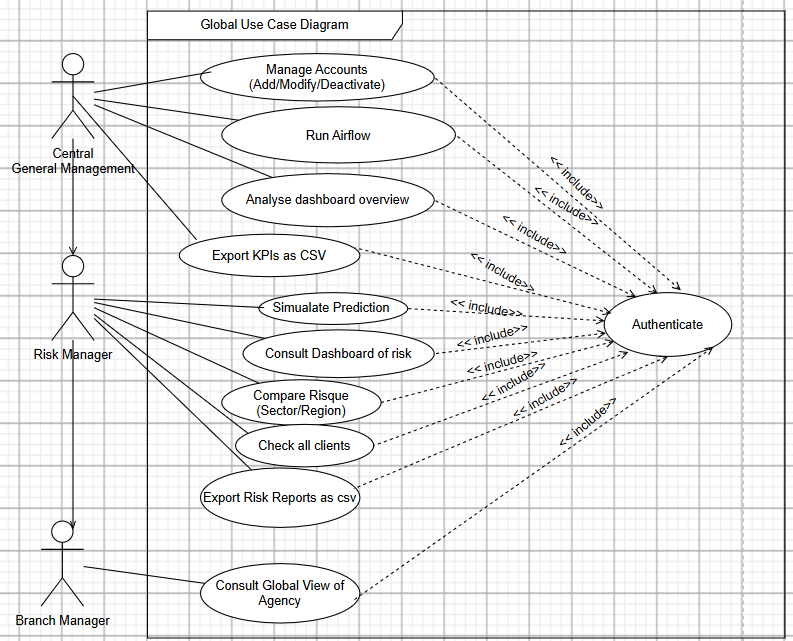
\includegraphics[width=0.9\textwidth]{figures/GlobalUseCaseDiagram.png}
\caption{Global Use case diagram\cite{atb_use_case_global}}
\label{fig:uc_sprint1}
\label{fig:atb_use_case_global}
\end{figure}

%================================================
\section{Project Planning}
%================================================

%----------------------------------------------
\subsection{Team and Roles}
%----------------------------------------------

The Scrum methodology having been adopted as detailed in Chapter~1, this section presents
the project team organisation for the ATB BI platform.

\begin{table}[H]
\centering
\caption{Scrum team organisation for the ATB BI platform}
\label{tab:atb_project_roles}
\begin{tabular}{|p{3.5cm}|p{3.8cm}|p{6.2cm}|}
\hline
\rowcolor{blue!15}
\textbf{Scrum Role} & \textbf{Assigned to} & \textbf{Responsibility} \\
\hline
Product Owner & ATB Administration (\textit{Direction March\'{e} Entreprises}) &
Represents business needs; prioritises the backlog; validates KPIs, risk views,
dashboard scope, and compliance requirements. \\
\hline
Scrum Master & M. Mouhamed Saddek Snoussi & Facilitates Scrum ceremonies, follows sprint
progress, removes blockers, and ensures alignment between the team and ATB stakeholders. \\
\hline
Development Team & Ahmed El Abed & Implements the platform end-to-end: ingestion, SQL
Server schemas, dbt models, Airflow DAGs, ML training (XGBoost and Random Forest), MLflow,
and Streamlit dashboards. \\
\hline
\end{tabular}
\end{table}

%----------------------------------------------
\subsection{Three-Tier Software Architecture}
\label{sec:atb_three_tier_architecture}
%----------------------------------------------

To ensure the modularity, maintainability, and scalability of the ATB platform, a
\textbf{three-tier software architecture} is adopted. This proven design pattern separates
the application into three distinct logical layers:

\begin{figure}[H]
\centering
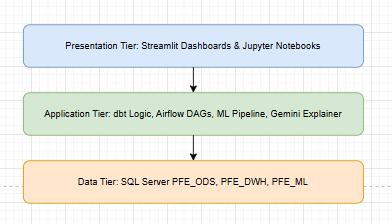
\includegraphics[width=0.75\textwidth]{atb_three_tier_architecture.png}
\caption{Three-tier software architecture of the ATB BI platform}
\label{fig:atb_three_tier_architecture}
\end{figure}

\textbf{1.~The Presentation Tier}: the Streamlit dashboard. Displays KPIs, interactive
charts, risk tables, model metrics, alerts, role-based pages, and AI-generated chart
explanations for ATB business users.

\textbf{2.~The Application Tier}: all processing and business logic. Includes Airflow DAGs
for daily scheduling, dbt transformation models (staging, intermediate, warehouse), risk
scoring SQL logic, Python ML scripts (XGBoost), MLflow integration, SHAP
explainability, and Gemini explanation calls.

\textbf{3.~The Data Tier}: persistent storage in SQL Server using three schemas:
\texttt{PFE\_ODS} for raw operational data (7 source tables), \texttt{PFE\_DWH} for the
constellation warehouse (8 dimensions, 2 fact tables, 281,960 total rows, 0 null foreign
keys), and \texttt{PFE\_ML} for ML prediction outputs.
%----------------------------------------------
\subsection{Product Backlog}
%----------------------------------------------

The product backlog groups all User Stories of the project, formulated according to the
Scrum standard. Each User Story is written from the perspective of one of the three
identified system actors, translating a concrete business need into a prioritised
functionality.

\begin{table}[H]
\centering
\caption{Product Backlog (Final Version - Streamlit \& AI)}
\label{tab:atb_product_backlog}

\small
\renewcommand{\arraystretch}{1.4}

\begin{tabularx}{\textwidth}{|c|c|c|X|}
\hline
\rowcolor{blue!15}
\textbf{US} & \textbf{Priority} & \textbf{Sprint} & \textbf{Description} \\
\hline

US 01 & Low & Sprint 1 &
As All Actors, I want to authenticate securely to access the platform. \\
\hline

US 02 & Medium & Sprint 1 &
As Central General Management, I want to create, modify, activate or deactivate accounts for branch and risk managers. \\
\hline

US 03 & Very High & Sprint 2 &
As Central General Management, I want to orchestrate the entire application automatically  with Airflow. \\
\hline

US 04 & High & Sprint 3 &
As Central General Management, I want to extract and load via Airbyte. \\
\hline

US 05 & High & Sprint 3 &
As Central General Management, I want to define and calculate risk KPIs in the central data warehouse. \\
\hline

US 06 & High & Sprint 3 &
As Branch Manager, I want to consult my agency's filtered view on Streamlit to monitor my activity. \\
\hline

US 07 & High & Sprint 3 &
As Central General Management, I want to analyze indicators for all agencies at the national level on Streamlit. \\
\hline

US 08 & High & Sprint 3 &
As Central General Management, I want to export and download management indicators as CSV files. \\
\hline

US 09 & Low & Sprint 3 &
As Risk Manager, I want to track the history and evolution of customers across all agencies. \\
\hline

US 10 & High & Sprint 4 &
As Risk Manager, I want to train the Artificial Intelligence algorithm to detect future defaults. \\
\hline

US 11 & High & Sprint 4 &
As Risk Manager, I want to consult the Artificial Intelligence predictions. \\
\hline

US 12 & High & Sprint 4 &
As Risk Manager, I want to read the automatic (AI-generated) interpretation of curves and the risk matrix on Streamlit. \\
\hline

US 13 & High & Sprint 4 &
As Risk Manager, I want to mathematically compare risk levels by sector and by geographic zone. \\
\hline

US 14 & High & Sprint 4 &
As Risk Manager, I want to download predictive customer scores (CSV) for other external tools. \\
\hline

\end{tabularx}
\end{table}

\clearpage
%----------------------------------------------
\subsection{Delivery Process (Releases)}
%----------------------------------------------

The project is structured into \textbf{3 Releases} covering \textbf{4 Sprints} of three
weeks each, consistent with the Gantt chart defined in Chapter~1.
Table~\ref{tab:atb_releases_plan} summarises how each release maps to sprints,
methodologies and user stories.

\begin{table}[!ht]
\centering
\caption{Delivery strategy: Releases, Sprints, and User Stories}
\label{tab:atb_releases_plan}
\renewcommand{\arraystretch}{1.35}
\footnotesize
\resizebox{\textwidth}{!}{
\begin{tabular}{|c|c|p{4.0cm}|p{7.0cm}|}
\hline
\rowcolor{blue!15}
\textbf{Release} & \textbf{Sprint(s)} & \textbf{Theme} & \textbf{User Stories} \\
\hline

\textbf{Release 1}
& \textbf{Sprint 1 \& 2}
& \textbf{Application \& \newline Engine}
&
\textbf{Sprint 1:} \newline
\textbf{US 01} : Authenticate securely to access the platform \newline
\textbf{US 02} : Create, modify, activate or deactivate accounts for branch and risk managers \newline
\textbf{Sprint 2:} \newline
\textbf{US 03} : Orchestrate the entire application automatically each night with Airflow \\
\hline

\textbf{Release 2}
& \textbf{Sprint 3}
& \textbf{Business \newline Intelligence (BI)}
&
\textbf{US 04} : Extract and load source files via Airbyte \newline
\textbf{US 05} : Define and calculate risk KPIs in the central data warehouse \newline
\textbf{US 06} : Consult my agency's filtered view on Streamlit to monitor my activity \newline
\textbf{US 07} : Analyze indicators for all agencies at the national level on Streamlit \newline
\textbf{US 08} : Export and download management indicators as CSV files \newline
\textbf{US 09} : Track the history and evolution of customers across all agencies \\
\hline

\textbf{Release 3}
& \textbf{Sprint 4}
& \textbf{Artificial \newline Intelligence (ML)}
&
\textbf{US 10} : Train the Machine learning algorithm to detect future defaults \newline
\textbf{US 11} : Consult the Machine learning predictions. \newline
\textbf{US 12} : Read the automatic (AI-generated) interpretation of curves and the risk matrix on Streamlit \newline
\textbf{US 13} : Mathematically compare risk levels by sector and by geographic zone \newline
\textbf{US 14} : Download predictive customer scores (CSV) for other external tools \\
\hline

\end{tabular}
}
\end{table}


%================================================
\section{Work Environment and Tools}
%================================================

The implementation of a banking BI and ML platform requires a stable technical environment
and a coherent technology stack.

%----------------------------------------------

\subsection{Hardware Environment}

The development, testing, transformation, dashboarding, and local ML training were performed
on a workstation with the following characteristics:

\begin{itemize}
    \item \textbf{Product Name}: MSI GF63 Thin 10SCXR
    \item \textbf{Operating System}: Microsoft Windows 10 Professionnel 64-bit (OS build 19045.6466)
    \item \textbf{BIOS Version}: E16R4IMS.107 (Release Date: 2020/05/28)
    \item \textbf{Processor}: Intel(R) Core(TM) i7-10750H CPU @ 2.60\,GHz
    \item \textbf{Memory (RAM)}: 16\,GB DDR4-2667 (Crucial CT16G4SFD8266.C16FD1) @ 1333\,MHz
    \item \textbf{Graphics}: NVIDIA GeForce GTX 1650 with Max-Q Design (4095\,MB) and Intel(R) UHD Graphics (1024\,MB)
\end{itemize}

\begin{figure}[H]
\centering

\includegraphics[height=1.8cm, keepaspectratio]{msi_logo.png}
\caption{MSI Logo\cite{msi_logo_atb}}
\label{fig:msi_logo_atb}
\end{figure}

This configuration provides sufficient CPU parallelism for dbt transformations, local four-model
ML training, Docker-based Airflow execution, and Streamlit dashboard development.


\subsection{Design and Development Tools}

\subsubsection{Visual design tools}

Architecture diagrams, warehouse models, UML use case diagrams, and report figures were designed
using \textbf{Draw.io} (diagrams.net) \cite{drawio}. This open-source tool is appropriate for
UML diagrams, BI architecture diagrams, and data flow representations. The editable source file for all the diagrams.

\begin{figure}[H]
\centering

\includegraphics[height=1.5cm, keepaspectratio]{drawio_logo.png}
\caption{Draw.io logo\cite{drawio}}
\label{fig:drawio_logo_atb}
\end{figure}

\subsubsection{Integrated development environment}

The codebase is organised and edited using \textbf{Visual Studio Code (VS Code)} \cite{vscode}.
It is suitable for Python development, SQL and dbt modelling, Airflow DAG editing, Markdown
documentation, and Git-based project organisation.

\begin{figure}[H]
\centering

\includegraphics[height=1.5cm, keepaspectratio]{vscode_logo.png}
\caption{Visual Studio Code logo\cite{vscode}}
\label{fig:vscode_logo_atb}
\end{figure}

\subsubsection{Version control}

Source code, dbt models, Airflow DAGs and report assets are versioned with
\textbf{Git}, managed through \textbf{GitHub Desktop} for day-to-day commits,
branching and synchronisation with the remote repository. This keeps the
pipeline reproducible and supports collaborative review across the three
releases.

\begin{figure}[H]
\centering

\includegraphics[height=1.5cm, keepaspectratio]{github_desktop.png}
\caption{GitHub Desktop\cite{github_desktop}}
\label{fig:github_desktop_logo_atb}
\end{figure}

\subsection{Technological Choices: Backend, Data and Machine Learning}

The central programming language of the project is \textbf{Python (version 3.8+)}, chosen for
its dominance in the data science and machine learning ecosystem.

\textbf{1. Data Storage and Database}
\begin{itemize}
    \item \textbf{Microsoft SQL Server}: central database engine used for all schemas
    \item \textbf{SQL Server Management Studio (SSMS)}: used for database inspection, query
    validation, schema verification, and manual checks.
\end{itemize}

\begin{figure}[H]
\centering

\includegraphics[height=1.4cm, keepaspectratio]{sqlserver_logo.png}
\caption{Microsoft SQL Server logo\cite{sqlserver_logo}}
\label{fig:sqlserver_logo_atb}
\end{figure}

\textbf{2. Data Ingestion and Transformation}

\textbf{Airbyte} is used as the ingestion orchestration layer for loading CSV sources into SQL Server.

\begin{figure}[H]
\centering

\includegraphics[height=1.5cm, keepaspectratio]{figures/airbyte.png}
\caption{Airbyte logo\cite{airbyte_logo}}
\label{fig:airbyte_logo_atb}
\end{figure}
\FloatBarrier

\textbf{Python} supports direct CSV loading, validation utilities, ML scripts, and dashboard services.

\begin{figure}[H]
\centering

\includegraphics[height=1.5cm, keepaspectratio]{figures/python.png}
\caption{Python logo\cite{python_logo}}
\label{fig:python_logo_atb}
\end{figure}
\FloatBarrier

\textbf{dbt (data build tool)} provides versioned SQL transformations and automated tests across
staging, intermediate, and warehouse layers.
\begin{figure}[H]
\centering

\includegraphics[height=1.5cm, keepaspectratio]{figures/dbt.png}
\caption{dbt logo\cite{dbt_logo}}
\label{fig:dbt_logo_atb}
\end{figure}
\FloatBarrier


\textbf{3. Orchestration and Infrastructure}
\begin{itemize}
    \item \textbf{Apache Airflow}: DAG definition, task dependencies, retries, and data quality
    checks on a daily schedule (02:00 UTC).
\begin{figure}[H]
\centering

\includegraphics[height=1.4cm, keepaspectratio]{figures/airflow.png}
\caption{Apache Airflow\cite{airflow_logo}}
\label{fig:airflow_logo_atb}
\end{figure}
\FloatBarrier

    \item \textbf{Docker}: containerisation platform used to deploy Airflow, Airbyte, and
    the Streamlit dashboard as isolated, reproducible services via Docker Compose.
\begin{figure}[H]
\centering
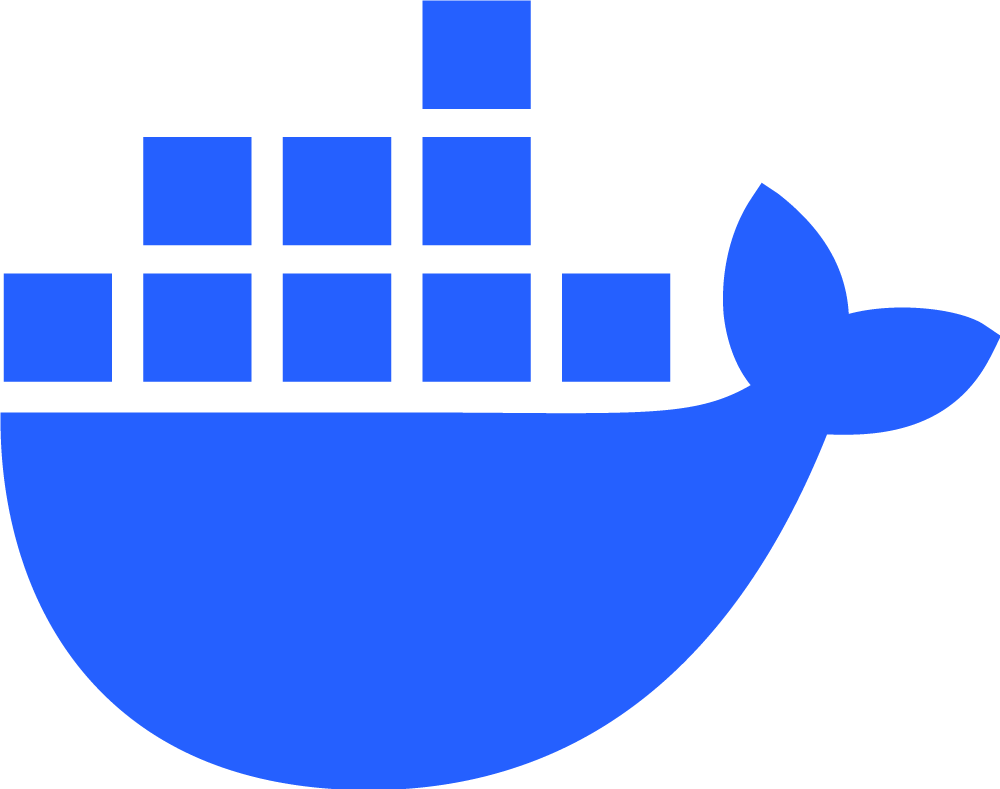
\includegraphics[height=1.4cm, keepaspectratio]{figures/docker.png}
\caption{Docker\cite{docker_logo}}
\label{fig:docker_logo_atb}
\end{figure}
\FloatBarrier
\end{itemize}

\textbf{4. Machine Learning}
\begin{itemize}
    \item \textbf{Scikit-learn}: preprocessing pipelines, metrics, \textbf{Random Forest},
    \textbf{Extra Trees}, \textbf{Logistic Regression}, and model selection utilities
    \cite{breiman2001, hastie2009}.
    \item \textbf{XGBoost}: primary customer risk classifier \cite{chen2016}.
    \item \textbf{MLflow}: experiment tracking, model registry, and production model traceability
    \cite{zaharia2018}.
\end{itemize}

\begin{figure}[H]
\centering
\includegraphics[height=1.5cm, keepaspectratio]{figures/mlflow.png}
\caption{MLflow tool logo\cite{mlflow_logo}}
\label{fig:ml_logos_atb}
\end{figure}
\FloatBarrier

\subsection{Technological Choices: Frontend, Visualisation and Data Analysis}
\begin{itemize}
    \item \textbf{Streamlit}: main operational dashboard framework, selected for rapid
    Python-based BI and ML integration \cite{bhatt2021}.
\begin{figure}[H]
\centering

\includegraphics[height=1.4cm, keepaspectratio]{figures/streamlit.png}
\caption{Streamlit\cite{streamlit_logo}}
\label{fig:streamlit_logo_atb}
\end{figure}
\FloatBarrier

    \item \textbf{Jupyter Notebooks}: ML model development, exploratory data analysis,
    feature engineering, and model selection reporting.
\begin{figure}[H]
\centering

\includegraphics[height=1.4cm, keepaspectratio]{figures/jupyter.png}
\caption{Jupyter Notebooks\cite{jupyter_logo}}
\label{fig:jupyter_logo_atb}
\end{figure}
\FloatBarrier

    \item \textbf{Google Gemini (gemini-2.0-flash)}: generative AI API used to explain dashboard
    charts in plain English for banking business users \cite{gemini2024}.
\end{itemize}



\begin{figure}[H]
\centering

\includegraphics[height=1.4cm, keepaspectratio]{figures/gemini.png}
\caption{Google Gemini\cite{gemini_logo}}
\label{fig:gemini_logo_atb}
\end{figure}
\FloatBarrier

%================================================
\section{Conclusion}
%================================================

This chapter established the theoretical, architectural, and functional foundations of the
ATB BI project. The state-of-the-art review covered Business Intelligence in banking
\cite{chaudhuri2011, eckerson2010}, multidimensional modelling and warehouse design approaches
(Kimball, Inmon, and hybrid) \cite{kimball2013, inmon2005}, machine learning paradigms and
evaluation metrics \cite{mitchell1997, lessmann2015}, the three-pillar global risk score
(Equation~\ref{eq:global_risk_score}) with scientific justification \cite{fatf2012, bcbs2011},
MLOps with MLflow \cite{zaharia2018, sculley2015}, generative AI for dashboard explanation
\cite{gemini2024}, and the comparative positioning of reporting frameworks.

The project is situated at the intersection of three mature domains: BI, data warehousing,
and machine learning. It starts from seven raw banking CSV files, loads data into SQL Server,
transforms it with dbt across three layers, builds a constellation warehouse with 8 dimensions
and 2 fact tables (281,960 total rows, 0 null foreign keys), computes customer risk scores
through the weighted three-pillar formula, trains and compares four supervised ML models (XGBoost
selected with F1 = 95.5\%, Random Forest benchmark with F1 = 89.5\%), tracks experiments with
MLflow, and exposes outputs through Streamlit dashboards and Jupyter Notebooks.

The requirements specification identified 7 actor types, 6 functional modules, 7 non-functional
constraints, 11 user stories across 3 sprints and 3 releases, and the three-tier software
architecture governing the implementation. The next chapter presents the detailed design and
implementation of the ATB data pipeline, from ingestion and warehouse construction to machine
learning and reporting deployment.
